\documentclass[a4paper, 11pt]{article}
\usepackage[python,linenum]{mypackage}
\usepackage{amsmath}
\usepackage{graphicx}
\usepackage{geometry}
\geometry{scale=0.8}
\usepackage{hyperref}
\usepackage{enumitem}
\usepackage{color}

\setenumerate[1]{itemsep=0pt,partopsep=0pt,parsep=\parskip,topsep=0pt}
\setitemize[1]{itemsep=0pt,partopsep=0pt,parsep=\parskip,topsep=0pt}
\setdescription{itemsep=0pt,partopsep=0pt,parsep=\parskip,topsep=0pt}


\title{
\normalfont \normalsize
\textsc{School of Data and Computer Science, Sun Yat-sen University} \\ [25pt] %textsc small capital letters
\rule{\textwidth}{0.5pt} \\[0.4cm] % Thin top horizontal rule
\huge  E14 BP Algorithm (C++/Python)\\ % The assignment title
\rule{\textwidth}{2pt} \\[0.5cm] % Thick bottom horizontal rule
\author{17341015 Hongzheng Chen}
\date{\normalsize\today}
}

\begin{document}
\maketitle
\tableofcontents
\newpage
\section{Horse Colic Data Set}
The description of the horse colic data set (\url{http://archive.ics.uci.edu/ml/datasets/Horse+Colic}) is as follows:
\begin{figure}[ht]
\centering
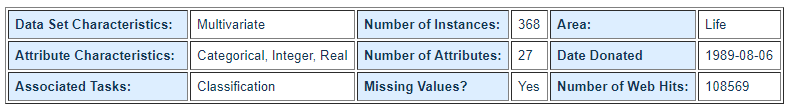
\includegraphics[width=15cm]{horse}
\end{figure}

We aim at trying to predict if a horse with colic will live or die.

Note that we should deal with missing values in the data! Here are some options:
\begin{itemize}
	\item Use the feature’s mean value from all the available data.
	\item Fill in the unknown with a special value like -1.
	\item Ignore the instance.
	\item Use a mean value from similar items.
	\item Use another machine learning algorithm to predict the value.
\end{itemize}

\section{Reference Materials}
\begin{enumerate}
	\item Stanford: \textbf{CS231n: Convolutional Neural Networks for Visual Recognition} by Fei-Fei Li,etc.
	\begin{itemize}
		\item Course website: \url{http://cs231n.stanford.edu/2017/syllabus.html}
		\item Video website: \url{https://www.bilibili.com/video/av17204303/?p=9&tdsourcetag=s_pctim_aiomsg}
	\end{itemize}

	\item \textbf{Machine Learning} by Hung-yi Lee
	\begin{itemize}
		\item Course website: \url{http://speech.ee.ntu.edu.tw/~tlkagk/index.html}
		\item Video website: \url{https://www.bilibili.com/video/av9770302/from=search}
	\end{itemize}
	\item A Simple neural network code template
\begin{lstlisting}
# -*- coding: utf-8 -*
import random
import math

# Shorthand:
# "pd_" as a variable prefix means "partial derivative"
# "d_" as a variable prefix means "derivative"
# "_wrt_" is shorthand for "with respect to"
# "w_ho" and "w_ih" are the index of weights from hidden to output layer neurons and input to hidden layer neurons respectively

class NeuralNetwork:
    LEARNING_RATE = 0.5
    def __init__(self, num_inputs, num_hidden, num_outputs, hidden_layer_weights = None, hidden_layer_bias = None, output_layer_weights = None, output_layer_bias = None):
    #Your Code Here

    def init_weights_from_inputs_to_hidden_layer_neurons(self, hidden_layer_weights):
    #Your Code Here

    def init_weights_from_hidden_layer_neurons_to_output_layer_neurons(self, output_layer_weights):
    #Your Code Here

    def inspect(self):
        print('------')
        print('* Inputs: {}'.format(self.num_inputs))
        print('------')
        print('Hidden Layer')
        self.hidden_layer.inspect()
        print('------')
        print('* Output Layer')
        self.output_layer.inspect()
        print('------')

    def feed_forward(self, inputs):
        #Your Code Here

    # Uses online learning, ie updating the weights after each training case
    def train(self, training_inputs, training_outputs):
        self.feed_forward(training_inputs)

        # 1. Output neuron deltas
        #Your Code Here
        # ∂E/∂zⱼ

        # 2. Hidden neuron deltas
        # We need to calculate the derivative of the error with respect to the output of each hidden layer neuron
        # dE/dyⱼ = Σ ∂E/∂zⱼ * ∂z/∂yⱼ = Σ ∂E/∂zⱼ * wᵢⱼ
        # ∂E/∂zⱼ = dE/dyⱼ * ∂zⱼ/∂
        #Your Code Here

        # 3. Update output neuron weights
        # ∂Eⱼ/∂wᵢⱼ = ∂E/∂zⱼ * ∂zⱼ/∂wᵢⱼ
        # Δw = α * ∂Eⱼ/∂wᵢ
        #Your Code Here

        # 4. Update hidden neuron weights
        # ∂Eⱼ/∂wᵢ = ∂E/∂zⱼ * ∂zⱼ/∂wᵢ
        # Δw = α * ∂Eⱼ/∂wᵢ
        #Your Code Here

    def calculate_total_error(self, training_sets):
        #Your Code Here
        return total_error

class NeuronLayer:
    def __init__(self, num_neurons, bias):

        # Every neuron in a layer shares the same bias
        self.bias = bias if bias else random.random()

        self.neurons = []
        for i in range(num_neurons):
            self.neurons.append(Neuron(self.bias))

    def inspect(self):
        print('Neurons:', len(self.neurons))
        for n in range(len(self.neurons)):
            print(' Neuron', n)
            for w in range(len(self.neurons[n].weights)):
                print('  Weight:', self.neurons[n].weights[w])
            print('  Bias:', self.bias)

    def feed_forward(self, inputs):
        outputs = []
        for neuron in self.neurons:
            outputs.append(neuron.calculate_output(inputs))
        return outputs

    def get_outputs(self):
        outputs = []
        for neuron in self.neurons:
            outputs.append(neuron.output)
        return outputs

class Neuron:
    def __init__(self, bias):
        self.bias = bias
        self.weights = []

    def calculate_output(self, inputs):
    #Your Code Here

    def calculate_total_net_input(self):
    #Your Code Here

    # Apply the logistic function to squash the output of the neuron
    # The result is sometimes referred to as 'net' [2] or 'net' [1]
    def squash(self, total_net_input):
    #Your Code Here

    # Determine how much the neuron's total input has to change to move closer to the expected output
    #
    # Now that we have the partial derivative of the error with respect to the output (∂E/∂yⱼ) and
    # the derivative of the output with respect to the total net input (dyⱼ/dzⱼ) we can calculate
    # the partial derivative of the error with respect to the total net input.
    # This value is also known as the delta (δ) [1]
    # δ = ∂E/∂zⱼ = ∂E/∂yⱼ * dyⱼ/dzⱼ
    #
    def calculate_pd_error_wrt_total_net_input(self, target_output):
    #Your Code Here

    # The error for each neuron is calculated by the Mean Square Error method:
    def calculate_error(self, target_output):
    #Your Code Here

    # The partial derivate of the error with respect to actual output then is calculated by:
    # = 2 * 0.5 * (target output - actual output) ^ (2 - 1) * -1
    # = -(target output - actual output)
    #
    # The Wikipedia article on backpropagation [1] simplifies to the following, but most other learning material does not [2]
    # = actual output - target output
    #
    # Alternative, you can use (target - output), but then need to add it during backpropagation [3]
    #
    # Note that the actual output of the output neuron is often written as yⱼ and target output as tⱼ so:
    # = ∂E/∂yⱼ = -(tⱼ - yⱼ)
    def calculate_pd_error_wrt_output(self, target_output):
    #Your Code Here

    # The total net input into the neuron is squashed using logistic function to calculate the neuron's output:
    # yⱼ = φ = 1 / (1 + e^(-zⱼ))
    # Note that where ⱼ represents the output of the neurons in whatever layer we're looking at and ᵢ represents the layer below it
    #
    # The derivative (not partial derivative since there is only one variable) of the output then is:
    # dyⱼ/dzⱼ = yⱼ * (1 - yⱼ)
    def calculate_pd_total_net_input_wrt_input(self):
    #Your Code Here

    # The total net input is the weighted sum of all the inputs to the neuron and their respective weights:
    # = zⱼ = netⱼ = x₁w₁ + x₂w₂ ...
    #
    # The partial derivative of the total net input with respective to a given weight (with everything else held constant) then is:
    # = ∂zⱼ/∂wᵢ = some constant + 1 * xᵢw₁^(1-0) + some constant ... = xᵢ
    def calculate_pd_total_net_input_wrt_weight(self, index):
    #Your Code Here

# An example:

nn = NeuralNetwork(2, 2, 2, hidden_layer_weights=[0.15, 0.2, 0.25, 0.3], hidden_layer_bias=0.35, output_layer_weights=[0.4, 0.45, 0.5, 0.55], output_layer_bias=0.6)
for i in range(10000):
    nn.train([0.05, 0.1], [0.01, 0.99])
    print(i, round(nn.calculate_total_error([[[0.05, 0.1], [0.01, 0.99]]]), 9))
\end{lstlisting}

\end{enumerate}
\section{Tasks}
\begin{itemize}
	\item Given the training set \texttt{horse-colic.data} and the testing set \texttt{horse-colic.test}, implement the BP algorithm and establish a neural network to predict if horses with colic will live or die. In addition, you should calculate the accuracy rate.
	\item Please submit a file named \texttt{E14\_YourNumber.pdf} and send it to \texttt{ai\_201901@foxmail.com}
\end{itemize}

\section{Codes and Results}
This experiment costs me three full days to finish (finetune the hyperparameters), but I still cannot figure out why my accuracy is so awkward. Sad :(

The following figure gives the training loss and the accuracy (without early stopping).
\begin{figure}[H]
\centering
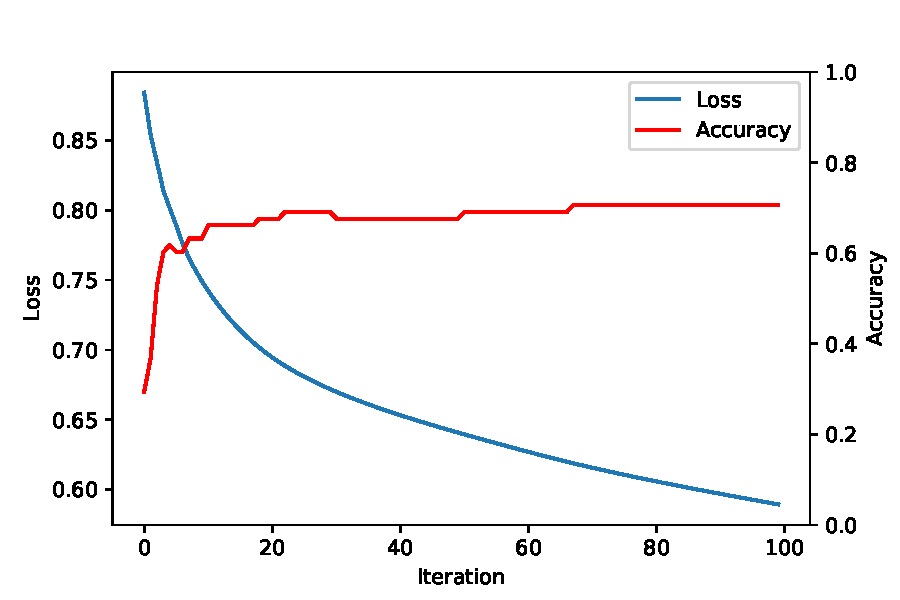
\includegraphics[width=0.6\linewidth]{fig/iteration.pdf}
\end{figure}

The training log is shown below (with early stopping), and the best accuracy I can get is 92\% accuracy on test set. (Notice the two figures are not in the same training process.)
\begin{figure}[H]
\centering
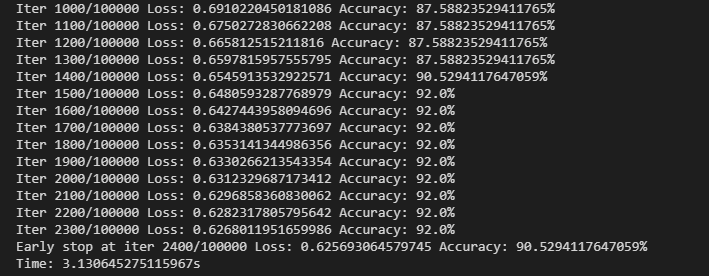
\includegraphics[width=0.8\linewidth]{fig/log.png}
\end{figure}

Please refer to \verb'nn.py' and \verb'bp.ipynb' (or the generated \verb'bp.py') for the codes.

Highlight some used techniques:
\begin{itemize}
    \item The network structure is $n_i$-$8$-$3$.
    \item Used Kaiming He's method to initialize the network
    \item A pytorch-like network class with \verb'forward' method is designed.
    \item L2-regulization and weight decay are used for training.
    \item All computation are based on tensor, and only the numpy package is used.
    \item \verb'np.einsum' is used for accelerating the tensor product in backpropagation.
    \item Heavy preprocessing methods are used, including one-hot encoding, missing data complement, and useless attributes removal. please refer to \verb'bp.ipynb' file for details.
    \item Early stopping is used to avoid overfitting, and learning rate decay is used for better convergence.
    \item Batch SGD is used to accelerate training.
    \item Checkpoints and logging make training more controlable.
\end{itemize}

Following gives the code of \verb'nn.py'.
\begin{lstlisting}
import numpy as np

class FullyConnectedLayer(object):
    """
    Linear transformation: y = x W^T + b
    Input: (N, in_features), i.e. a row vector, in this example, N = 1
    Output: (N, out_features)

    Attributes:
      Weight: (in_features, out_features)
      Bias: (out_features)

    Ref:
    http://cs231n.stanford.edu/vecDerivs.pdf
    """

    def __init__(self, in_features, out_features, bias=True):
        self.in_features = in_features
        self.out_features = out_features
        """
        Xavier initialization
        # https://www.deeplearning.ai/ai-notes/initialization/
        W^{[l]} &\sim \mathcal{N}(\mu=0,\sigma^2 = \frac{1}{n^{[l-1]}})
        b^{[l]} &= 0

        Kaiming He initialization
        # https://medium.com/@shoray.goel/kaiming-he-initialization-a8d9ed0b5899
        """
        self.weight = np.random.normal(0,np.sqrt(2/in_features),(out_features,in_features))
        if bias:
            self.bias = np.random.rand(out_features)
        else:
            self.bias = None

    def forward(self, inputs):
        """
        Forward propagation
        """
        if type(self.bias) != type(None):
            return np.dot(inputs, self.weight.T) + self.bias
        else:
            return np.dot(inputs, self.weight.T)

    def __call__(self,x):
        """
        Syntax sugar for forward method
        """
        return self.forward(x)

class Network(object):

    def __init__(self,in_features,hidden_features,out_features,learning_rate=0.01):
        """
        Here three-layer network architecture is used

        The number of neurons in each layer is listed below:
        in_features -> hidden_features -> out_features
        """
        self.fc1 = FullyConnectedLayer(in_features,hidden_features,True)
        self.fc2 = FullyConnectedLayer(hidden_features,out_features,True)
        self.learning_rate = learning_rate
        self.memory = {} # used for store intermediate results
        self.train_flag = True

    def train(self):
        """
        When training, memory is set to remember the intermediate results
        """
        self.train_flag = True

    def eval(self):
        """
        When inferencing, memory is no need to set
        """
        self.train_flag = False

    def relu(self,x):
        """
        Relu(x) = x, x > 0
                  0, x <= 0
        """
        return np.maximum(0,x)

    def d_relu(self,x):
        x[x <= 0] = 0
        x[x > 0] = 1
        return x

    def sigmoid(self,x):
        """
        Element-wise function
        \Sigma(x) = 1/(1+\ee^{-x})
        """
        return 1 / (1 + np.exp(-x))

    def d_sigmoid(self,x):
        """
        Derivative of sigmoid function
        \Sigma'(x) = \Sigma(x) * (1 - \Sigma(x))
        """
        return self.sigmoid(x) * (1 - self.sigmoid(x))

    def tanh(self,x):
        return np.tanh(x)

    def d_tanh(self,x):
        return 1 - np.tanh(x) ** 2

    def MSE(self,y_hat,y):
        """
        Mean-square error (MSE)
        """
        return np.linalg.norm(y_hat - y) # 2-norm

    def cross_entropy(self,y_hat,y):
        """
        Cross entropy loss
        """
        return y * np.log(y_hat) + (1 - y) * np.log(1 - y_hat)

    def forward(self,x):
        """
        w/o activation: z^{(l+1)} = W^{(l)}a^{(l)} + b^{(l)}
        w/ activation : a^{(l+1)} = f(z^{(l+1)})
        """
        # training
        if self.train_flag:
            self.memory["a0"] = np.copy(x)
            x = self.fc1(x) # N * hidden
            self.memory["z1"] = np.copy(x)
            x = self.sigmoid(x)
            self.memory["a1"] = np.copy(x)
            x = self.fc2(x) # N * out
            self.memory["z2"] = np.copy(x)
            x = self.sigmoid(x)
        # inferencing
        else:
            x = self.fc1(x) # N * hidden
            x = self.sigmoid(x)
            x = self.fc2(x) # N * out
            x = self.sigmoid(x)
        return x

    def backward(self,y_hat,y,lamb=0):
        """
        Use Mean-Squared Error (MSE) as error function

        lambda is used for weight decay

        Ref: http://ufldl.stanford.edu/tutorial/supervised/MultiLayerNeuralNetworks/
        """
        batch_size = y.shape[0]
        # Calculate \delta
        # output layer: \delta(n_l) = -(y - a(n_l)) * f'(z(n_l))
        # other layers: \delta(l) = W(l)^T\delta(l+1) * f'(z(l))
        delta = [0] * 3
        delta[2] = (y_hat - y) * self.d_sigmoid(self.memory["z2"]) # N * out_features
        delta[1] = np.dot(delta[2],self.fc2.weight) * self.d_sigmoid(self.memory["z1"]) # N * hidden_features
        # print(delta[2].shape,delta[1].shape)

        # Calculat \nabla
        # output layer: \nabla_{W(l)}J(W,b;x,y) = \delta(l+1)(a(l))^T # outer product
        # other layers: \nabla_{b(l)}J(W,b;x,y) = \delta(l+1)
        nabla_W = [0] * 2
        nabla_W[1] = np.einsum("ij,ik->ijk",delta[2],self.memory["a1"]) # N * out_features * hidden_features
        nabla_W[0] = np.einsum("ij,ik->ijk",delta[1],self.memory["a0"]) # N * hidden_features * in_features
        nabla_b = [0] * 2
        nabla_b[1] = delta[2] # N * out_features
        nabla_b[0] = delta[1] # N * hidden_features
        # print(nabla_W[1].shape,nabla_W[0].shape,nabla_b[1].shape,nabla_b[0].shape)

        # Update parameters
        # W(l) = W(l) - \alpha((1/m \Delta W(l)) + \lambda W(l))
        # b(l) = b(l) - \alpha(1/m \Delta b(l))
        # Use einsum to accelerate
        # https://rockt.github.io/2018/04/30/einsum
        nabla_W[1] = nabla_W[1].mean(axis=0)
        nabla_W[0] = nabla_W[0].mean(axis=0)
        nabla_b[1] = nabla_b[1].mean(axis=0)
        nabla_b[0] = nabla_b[0].mean(axis=0)

        # weight decay, lambda is the L2 regularization term
        self.fc2.weight -= self.learning_rate * (nabla_W[1] + lamb * self.fc2.weight / batch_size)
        self.fc1.weight -= self.learning_rate * (nabla_W[0] + lamb * self.fc1.weight / batch_size)
        self.fc2.bias -= self.learning_rate * nabla_b[1]
        self.fc1.bias -= self.learning_rate * nabla_b[0]
\end{lstlisting}

\end{document}